\setcounter{secnumdepth}{1}
\section{Einführung}
Diese Bachelorarbeit behandelt die Ausführung und Verarbeitung von asynchronen Prozessen in der Programmierung speziell in der Sprache Typescript.\\
Zielgruppe dieser Arbeit sind Personen, die Grundkenntnisse in der Sprache Javascript/Typescript vorweisen können.
Sollte man von der Skriptsprache Typescript noch nicht/kaum etwas gehört haben, sollte vor dem Lesen dieser Arbeit die offizielle Dokumentation von Microsoft durchgegangen werden.

\begin{center}
\url{https://www.typescriptlang.org/docs/home.html} 
\end{center}

In dieser Arbeit wird nur oberflächlich auf die Unterschiede der beiden Sprachen eingegangen. Des Weiteren sollte man von den Kernkonzepten der Promises und Observables schon mal gehört haben, da diese in der Arbeit gegenübergestellt werden.

\subsection{Typescript}
Typescript. Bereits der Name sagt schon was diese Sprache ausmacht. Sie \textit{(\glqq{}Type\grqq{} zu deutsch: Typ)} ist eine typisierte Form der Skriptsprache Javascript. In Typescript ist es Standard, jede Variable, Funktion und Funktionsparameter im Vorfeld zu typisieren. Mit dem Typescript Compiler werden Dateien mit dem Suffix *.ts in *.js überführt.

\subsubsection{Beispiel}

\begin{figure}[h!]
\begin{lstlisting}
class Greeter {
    greeting: string;
    constructor (message: string) {
        this.greeting = message;
    }
    greet() {
        return "Hello, " + this.greeting;
    }
}  
\end{lstlisting}
\caption{Typescript Klasse \cite{typescript-example}}
\end{figure}

Im oberen Code-Schnipsel wurden die variablen und die Klassenmethoden nach Typescript-Standard deklariert. Diese Typen werden beim übersetzen in Javascript ignoriert. Der Kompiler einer Entwicklungsumgebung prüft dann, ob beim übergeben eines Parameters in den Konstruktor ein numerischer oder Boolean-Wert eingesetzt wird. Dies wird dann als ein Fehler erkannt. Der Kompiler übersetzt auch nicht direkt deklarierte Typen. Wie in diesem Fall wird erkannt, dass die Methode greet() einen String-Wert zurückgibt.

\begin{figure}[t]
\begin{lstlisting}
var Greeter = (function () {
    function Greeter(message) {
        this.greeting = message;
    }
    Greeter.prototype.greet = function () {
        return "Hello, " + this.greeting;
    };
    return Greeter;
})(); 
\end{lstlisting}
\caption{Überführung in Javascript \cite{typescript-example}}
\end{figure}
In der vom Kompiler auf Javascript übersetzten Version werden die erstellten Klassen und Typen vollständig eliminiert. Was verbleibt ist die Übersetzung der Klassen-Methode greet() und des Konstruktors. Sowohl Klassen als auch Interfaces werden in Javascript nicht genutzt.

\subsubsection{Kompiler}

In einer tsconfig.json Datei können die Kompiler-Optionen für Typescript gesetzt werden. Zudem können Root-Dateien definiert und ausgeschlossen werden. Die Auflistung einer tsconfig.json Datei in einem Verzeichnis zeigt, dass das es sich hierbei um das Root-Verzeichnis des Projekts handelt. Ein Beispiel für die Konfiguration einer solchen Datei könnte folgend aussehen: 

\begin{figure}[h!]
\begin{lstlisting}
{
    "compilerOptions": {
        "module": "system",
        "noImplicitAny": true,
        "removeComments": true,
        "preserveConstEnums": true,
        "outFile": "../../built/local/tsc.js",
        "sourceMap": true
    },
    "include": [
        "src/**/*"
    ],
    "exclude": [
        "node_modules",
        "**/*.spec.ts"
    ]
}  
\end{lstlisting}
\caption{tsconfig.json \cite{tsconfig}}
\end{figure}
Hier kann z.B. mit der Regel 
\glqq noImplicitAny\grqq{} festgelegt werden, dass Methoden als auch Parameter und Variablen getypt werden müssen bei ihrer Deklaration. Sind sie nicht getypt: Bedeutet dies für den Kompiler sie sind als any deklariert.
Die Konfiguration dieser Datei betrifft Kompilier-Fehler. Fehler zur Laufzeit sind von der Konfiguration ausgeschlossen.
Zudem wird in jedem Fall eine Javascript-Datei erstellt, auch der Compiler einen Fehler anzeigen. Diese Datei ist potenziell auch lauffähig.\\\\

Da Syntaktisch alles was auf Javascript geschrieben auch valider Typescript Code ist, kann man Typescript als Superset von Javascript bezeichnen. Demzufolge kann man die Nutzung von statische Typen, Klassen und Interfaces als Konvention betrachten.

Im Laufe der Zeit findet Typescript immer mehr Beliebtheit in Unternehmensprojekten. Entwicklerteams können durch die Typisierung schneller Bugs am Code erkennen und durch den modularen Aufbau, den Typescript ermöglicht, die Organisation und Dokumentation von großen Projekten verbessern. Diese Tendenz wird von der beliebten Entwicklerplattform Stackoverflow untermauert, die laut einer Umfrage welche die beliebtesten Programmiersprachen der Entwickler sei, folgendes rausgekommen ist:

\begin{figure}[H]
\centering
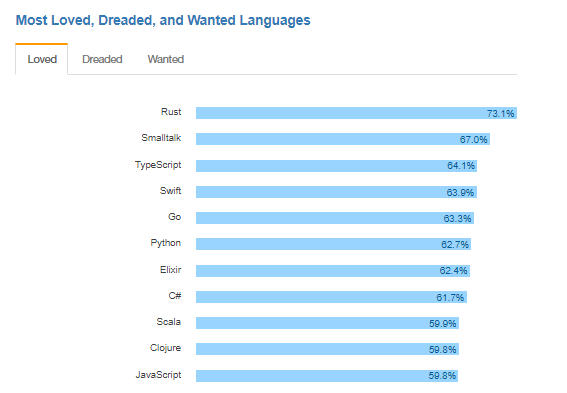
\includegraphics[height=6cm]{stackoverflow-typescript-popularity}
\caption{Prozentualer Anteil der Entwickler die Interesse an neuen Technologien zeigen und weiter mit neuen Technologien arbeiten möchten. Jahr: 2017 \cite{typescript-survey}}
\end{figure}

\subsection{Aufbau}
Diese Bachelorarbeit wird aus zwei Code-Projekten bestehen. Während das ersten Projekt nur im Kern die Ausführung von asynchronen Verarbeitungsprozessen präsentiert (mit der Hilfe von simulierten Anwendungsbeispielen), wird das zweite Projekt eine Singlepage-Applikation darstellen und praxisnahe Beispiele anwenden. Dies soll mit dem Framework Angular und Google Firebase als DaaS bewerkstelligt werden. Das zweite Projekt wird im zweiten Teil der Arbeit vorgestellt. Die Repositories für beide Projekte sind zu finden unter: 

\begin{center}
\url{https://github.com/MarcoLeko/Promises-vs.-Observables.git} \\
\url{https://github.com/MarcoLeko/Angular-Firebase-App.git}
\end{center}

\subsection{Zielsetzung}
Ziel der Arbeit ist die Betrachtung und Aufbereitung des Einsatzes von Sprachmitteln zur asynchronen Verarbeitung in Typescript in einer Form, die Einsteigern in die Thematik hilft, die unterschiedlichen Konzepte voneinander abzugrenzen und richtig einzusetzen. Dazu soll asynchrone Verarbeitung insgesamt anhand brauchbarer und für den Einsatz von Typescript typischer Szenarien motiviert werden. Es werden die zur Verfügung stehenden Sprachmittel Promises und Observables mit ihren jeweiligen Features vorgestellt. Dabei soll nach dem Vorstellen der beiden Kernkonzepte im zweiten Teil der Arbeit \glqq Best Practice\grqq{}-Beispiele vorgeführt werden. Nach dem Lesen dieser Arbeit soll der Leser ein gewisses Verständnis dafür gewonnen haben, welche der vorgestellten Sprachmitteln für welchen Anwendungsfall sinnvoller erscheint. 

\subsection{Terminologie}
Um die Abgrenzung von verschiedenen asynchronen Sprachmitteln zu beherrschen, muss vorerst geklärt werden, was Asynchronität bedeutet.\\\\
Der zentrale Teil eines Computers, welches Programme und einzelne Schritte zum Ausführen bringt, ist der Prozessor. Die Geschwindigkeit in der eine Schleife von einem Programm ausgeführt wird, hängt von der Geschwindigkeit des Prozessors ab. Programme interagieren jedoch mit Operationen außerhalb des Zuständigkeitsbereiches eines Prozessors, wie z.B. die Kommunikation über ein Netzwerk oder Abfragen von Daten von der Festplatte. Solche Operationen hängen von anderen Ressourcen ab und brauchen Zeit. In solchen Szenarien wäre es unvorteilhaft, wenn der Prozessor im Leerlauf stecken würde, anstatt andere Operationen in der Zwischenzeit auszuführen. Genau für solche Aufgaben ist das Betriebssystem da. Das Betriebssystem sorgt dafür, dass Kapazitäten des Prozessors auf parallel laufende Programme wechselt, während es auf die Antwort von ausgeführten Operationen wartet. Es entstehen dabei verschiedene \glqq Threads\grqq{}. Und hier kommt die Asynchronität ins Spiel:

\subsubsection{Asynchronität}
Ein \textbf{asynchrones} Programmiermodell erlaubt multiple Abläufe zum selben Zeitpunkt. Wenn eine Aktion ausgeführt wird, läuft das Programm in einem anderen \glqq Thread\grqq{} weiter. Sollte die Operation fertigt gestellt sein, wird das Programm informiert und liefert das Ergebnis zurück. Ein Beispiel dafür wäre das Suchen von Dateien auf einer Festplatte. \\

In einem \textbf{synchronen} Programmiermodell entstehen Abläufe nacheinander. Wenn eine Funktion mit einer zeitintensiven Aktion abgerufen wird, wird das Ergebnis erst nach dem Beenden der Operation zurückgegeben.  In diesem Zeitintervall werden keine Nebenoperationen ausgeführt. \\

Ein Beispiel zum Vergleich von synchronem- und asynchronem Programmieren: 
Die Wiedergabe mehrerer Meldungen in einem Browser:
*Source-code Beispiel*